% TEX STUDIO MAGIC-COMMAND
% !TeX document-id = {21ffa6e2-6c8f-4532-897c-386dc477f19a}
% !TeX root = abstract.tex
%%% ↑ TeXのファイル名にあわせること．
% !TeX encoding = utf8
% !TeX TXS-program:compile = lualatex -synctex=1 -interaction=nonstopmode -halt-on-error %.tex
% !TeX TXS-program:quick = txs:///compile | txs:///view-pdf-internal --embedded

%%%-------------------------------------------------------------------------
%%% PD3予稿集テンプレート （main.tex）
%%% 作成： 金沢工大・情報工学科・鷹合研究室(2022,01/12)
%%%-------------------------------------------------------------------------

%%%%%%%%%%%%%%%%%%%%%%%%%%%%%%%%%%%%%%%%%%%%%%%%%%%%%%%%%%%%%%%%%%%%%%%%%%%
%                               テーマ，著者情報をここに書き込んでください
%ここから ------------------------------------------------------------------

%%% テーマ番号
\def\THEMEID{SP-PS}

%%% タイトル
\def\TITLEJP{聴覚障害者向けの映像フィードバックを用いた\\発音練習アプリ} % 文字は変えず，「アプリ」の途中で改行されないよう改行の位置だけ決めている
\def\TITLEEN{A Pronunciation Practice App Using Video Feedback for People with Hearing Impairments}
\def\CENTERADJ{3.3} % ここを書き換えて，表紙の「プロジェクトテーマ」という文字列がセル中心になるよう調整してください

%%% 教員名
\def\PROFNAME{金道 敏樹 教授}

%%% アブストラクト（英文で書く）
% 最低：100ワード，最大：300ワード前後
% 英文部分については，句読点は半角にすること．つまり", "か". "を使う
\def\ABSTRACT{
People with hearing impairments find it difficult to check their own pronunciation by ear. We developed SP-PS, a pronunciation practice app with video feedback. It compares a learner's word utterance with a model video recorded by a family member or teacher, shows the differences in graphs and videos, and suggests how to correct them along with a score out of 100. The speech is segmented into morae by forced alignment with Julius, and pitch accent (50 points), mora duration (30 points) and vowel formants (20 points) are scored against the model. Lip-shape vectors from MediaPipe Face Mesh are aligned by dynamic time warping to measure the gap between voice and lips for each mora, and gaps beyond perceptual thresholds in the literature reduce the score by up to 5 points. In system tests, all 52 model words scored 100 against themselves, and injected audio-visual gaps were detected without false alarms under a tempo change. The detected accent nucleus, however, matched the dictionary accent type in only 15 of 45 words. A one-month study at a school for the deaf is planned.
}

%%% キーワード(5個まで)
\def\KEYWORDS{Pronunciation training，Hearing impairment，Video feedback，Pitch accent，Audio-visual synchrony}

%%% 著者リスト
\def\AUTHORS{
\begin{minipage}{13.5cm}
1300808~吉田 遥斗(YOSHIDA Haruto)      ~~~~~~ 1304695~宮丸 琉聖(MIYAMARU Ryusei)\\
1307713~前田 侑輝(MAEDA Yuki)
\end{minipage}
}

% テーマ，著者情報ここまで -----------------------------------------------------


%%%%%%%%%%%%%%%%%%%%%%%%%%%%%%%%%%%%%%%%%%%%%%%%%%%%%%%%%%%%%%%%%%%%%%%%%%%%
%                                本文
\documentclass{tkglabs}
\usepackage{amsmath}
\begin{document}
\maketitle
\begin{multicols*}{2} % *アスタ付きだとページのバランシングを無効にできる
%本文ここから ------------------------------------------------------------------

\section{はじめに}
聴覚に障害のある人は，自分の声を耳で確かめにくく，声と口の動きの協調が聴者と異なることも報告されている\cite{mcgarr1982}．
そのため，指導者が隣にいないと発音の練習を繰り返しにくい．

一方，話者の口が見えると，雑音の中でも言葉の聞き取りが大きく向上する\cite{sumby1954}．
聴覚障害児に口の動きを見せる訓練で，発音が改善したという報告もある\cite{massaro2004}．
しかし，発音学習支援システム\cite{neri2002}の多くは第二言語の学習者を対象とし，音声だけを評価する．
日本語のピッチと長さを視覚的に練習させるシステム\cite{hirata2004}も，学習者の口の動きは扱わない．

そこで本プロジェクトでは，聴覚障害者向けの映像フィードバックを用いた発音練習アプリ SP-PS を開発した．
図\ref{FIG_CONCEPT}にコンセプトを示す．家族などが録画したお手本と学習者の音程（声の高さ）や口の動きを比べ，違いをグラフや動画で示したうえで，「最初の音程を低く」のように直し方（解決策）を提案する．
本稿では評価手法とアプリの検証結果を報告する．

%%%%%%%%%%%%%%%%%%%%%%%%%%%%%%%%%%%%%
\begin{figure} % 小さな図（コンセプトペーパーのイラスト）
	\centering
	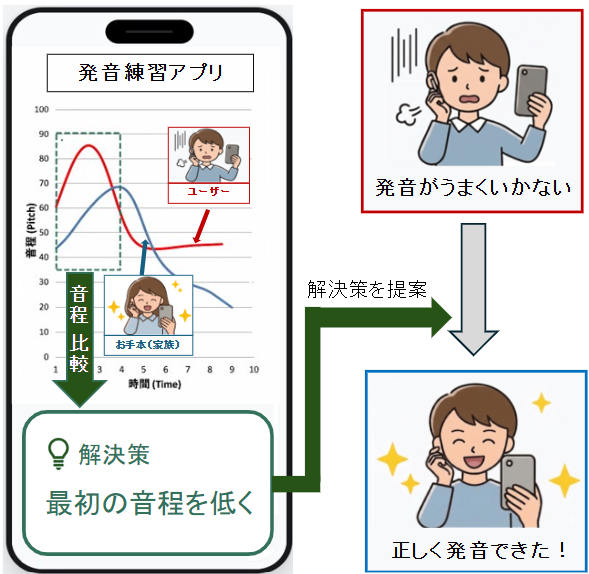
\includegraphics[width=0.86\linewidth]{fig/concept.png}
	\vspace{6mm}
	\figcap{本アプリのコンセプト}{Concept of the app}{FIG_CONCEPT}
\end{figure}

\section{アプリの構成}
\subsection{処理の流れ}
単語を登録するとき，家族や先生がその単語を発音する様子を3秒間録画し，その動画からお手本の音声と口の動きを取り込む．
学習者はスマートフォンのブラウザで，お手本の動画を見てから録音と口元の録画を行う．結果は◎○△と「つぎは，ここだけ」で示し，苦手な音のドリルを提案する．

音声は Julius\cite{lee2009}の強制アライメントでモーラ（拍）ごとに区切り，Praat の自己相関法\cite{boersma1993}で基本周波数（F0）を，同じく Praat でフォルマントを測る．
映像からは MediaPipe Face Mesh\cite{kartynnik2019}で唇の輪郭の20点を取り出し，両目の外側の端の距離で割った20次元の唇形状ベクトルとする．


\subsection{発音の評価}
合計点 $S$ は，アクセント $S_{\mathrm{A}}$（50点）・モーラ長 $S_{\mathrm{D}}$（30点）・母音品質 $S_{\mathrm{V}}$（20点）の和から，口と声のタイミングの減点 $P_{\mathrm{AV}}$（0〜5点）を引いたものである．
\begin{equation}
S = \mathrm{clip}\bigl(S_{\mathrm{A}} + S_{\mathrm{D}} + S_{\mathrm{V}} - P_{\mathrm{AV}},\ 0,\ 100\bigr)
\end{equation}

\textbf{アクセント}：日本語はピッチアクセントの言語で，音が下がる位置（アクセント核）が語の区別に関わる．
F0 を話者ごとの中央値を基準とした半音に直し，録音をお手本の時間軸に音素ごとに伸縮させてから比べる．
核の位置 $S_{\mathrm{nuc}}$，ピッチの Pearson 相関 $S_{\mathrm{cor}}$，各モーラの高低（H/L）の一致率 $S_{\mathrm{HL}}$，モーラ内の揺れ $S_{\mathrm{stb}}$（各0〜60）を重み付けして合わせる．
\begin{equation}
\tilde{S}_{\mathrm{A}} = 0.40 S_{\mathrm{nuc}} + 0.28 S_{\mathrm{cor}} + 0.22 S_{\mathrm{HL}} + 0.10 S_{\mathrm{stb}}
\end{equation}
とし，$S_{\mathrm{A}} = \min(50,\ \tfrac{5}{6}\tilde{S}_{\mathrm{A}} + 3)$ とする．

\textbf{モーラ長}：各モーラの長さが発話全体に占める割合 $\eta_g$（\%）をお手本と比べるので，全体の速さには左右されない．
長音・促音は意味の区別に関わるので重み $w_g = 2.0$，撥音は1.5，その他は1.0とする．
\begin{equation}
S_{\mathrm{D}} = \tfrac{3}{4}\max\Bigl(0,\ 40\Bigl(1 - \frac{\sum_g w_g \lvert \eta^{\mathrm{ref}}_g - \eta^{\mathrm{lrn}}_g \rvert}{\bar{\eta}\sum_g w_g}\Bigr)\Bigr)
\end{equation}
$\bar{\eta} = 100/G$（$G$ はモーラ数）で割り，モーラ数による差をなくした．

\textbf{母音品質}：各モーラの区間の30・50・70\%の時刻で第1・第2フォルマント（$F_1$, $F_2$）を測り，その中央値を Bark 尺度 $z(\cdot)$\cite{traunmuller1990}に直して距離を求める．
話者の声道の長さの違いは，同じ位置のモーラの $F_1$・$F_2$ の比の中央値 $\gamma$（0.80〜1.25）で補正する．
\begin{equation}
\delta_g = \sqrt{\Bigl(\tfrac{z(\gamma F^{\mathrm{ref}}_{1,g}) - z(F^{\mathrm{lrn}}_{1,g})}{3}\Bigr)^2 + \Bigl(\tfrac{z(\gamma F^{\mathrm{ref}}_{2,g}) - z(F^{\mathrm{lrn}}_{2,g})}{4}\Bigr)^2}
\end{equation}
重み付き平均 $\bar{\delta}$ から $S_{\mathrm{V}} = \mathrm{clip}(20 e^{-\bar{\delta}}, 0.5, 20)$ とする．


\subsection{口と声のタイミングの照合}
声と口のどちらか一方だけがずれる誤りは，片方の情報だけでは見つけられない．そこで，お手本と学習者の唇形状ベクトルの系列を FastDTW\cite{salvador2007}で対応付け，お手本のモーラの中心時刻を学習者の映像の時刻 $\tau^{\mathrm{v}}_k$ に写す．
これを音声のアライメントが示す時刻 $\tau^{\mathrm{a}}_k$ と比べ，ずれ $\Delta_k = \tau^{\mathrm{v}}_k - \tau^{\mathrm{a}}_k$ を求める．
録画開始のタイミングの機材差を除くため，発話全体の中央値からの差 $\tilde{\Delta}_k$ を使う．

人がずれに気づく範囲は，声が先のとき約45\,ms，口が先のとき約200\,msと非対称である\cite{grant2003}．
また，ずれが400\,msになると，口が見えることによる聞き取りの向上はほぼ失われる\cite{grant2001}．
これに合わせ，モーラごとの損失 $\lambda_k$ と減点を次のように定めた．
\begin{equation}
\lambda_k = \mathrm{clip}\Bigl(\frac{\lvert \tilde{\Delta}_k \rvert - \theta_k - \varepsilon}{400\,\mathrm{ms} - \theta_k},\ 0,\ 1\Bigr)
\end{equation}
減点は $P_{\mathrm{AV}} = 5 \cdot \frac{1}{K}\sum_k \lambda_k$ である．
$\theta_k$ は声が先なら45\,ms，口が先なら200\,ms，$\varepsilon$ はコマの間隔による誤差，$K$ は比べたモーラ数である．

\section{評価実験の方法}
学校での調査の前に，(1)お手本52語（人の録音30語，合成音声22語）の自己比較，(2)人工的なずれを加えた口と声の照合の校正，(3)アクセント型の分かっている45語での核の検出を行った．

\section{実験結果}
\textbf{自己比較}：52語すべてが100点となり，誤ったフィードバックは出なかった．

\textbf{口と声の照合}：表\ref{TBL_SYNC}に結果を示す．
一様なずれは中央値に現れ，中央値からの差のばらつき（中央絶対偏差）は増えなかった．テンポ1.5倍でも誤検出はなく，局所的なずれはばらつきに現れた．

%%%%%%%%%%%%%%%%%%%%%%%%%%%%%%%%%%%%%
\begin{table} % 小さな表
	\centering
	\tabcap{口と声の照合の校正}{Calibration of the audio-visual check}{TBL_SYNC}
	\tabcolsep = 3pt
	\begin{tabular}{lrr}
		\Hline
		加えたずれ [ms] & 中央値 [ms] & ばらつき [ms]\\
		\hline
		なし（自己一致） & $\pm 11$以内 & 2〜9\\
		一様 50/100/200 & $-61$/$-111$/$-211$ & ---\\
		テンポ1.5倍 & --- & 8\\
		後半のみ $+150$ & --- & 75\\
		\Hline
	\end{tabular}
\end{table}

\textbf{アクセント核}：検出した核が辞書のアクセント型と一致したのは45語中15語であった（下降のしきい値を0.25〜2.0半音で変えても11〜22語）．



\section{考察}
同じ発音は満点となり，口と声のずれを録画開始の機材差と分けて検出できることを確かめた．

一方，アクセント核の検出は辞書のアクセント型とあまり一致しなかった．
単語を単独で発音すると，平板型でも語末で声が大きく下がり，それを核と取り違えるためである．
また，重みやしきい値は開発時に決めた値で，点数と人の評価の一致は未検証である．口と声の範囲も健聴者が英語を見聞きした実験の値であり，生徒の日本語の発話への当てはまりは今後の課題である．

\section{まとめ}
聴覚障害者が一人で発音を練習できるよう，映像フィードバックを用いた発音練習アプリ SP-PS を開発した．
3観点の評価と口と声のタイミングの照合を実装し，動作を確かめた．
今後，聴覚特別支援学校の中学部・高等部の生徒に約1か月使ってもらい，発音の改善がみられるかと，使いやすさについての意見を調べる．

%% 参考文献（必要に応じて追加）%%%%%%%%%%%%%%%%%%%%%%%%%%%%%%%%%%
% 古典的な方法使う場合
\begin{thebibliography}{99}
\bibitem{mcgarr1982} N. S. McGarr, A. L{\"o}fqvist, ``Obstruent production by hearing-impaired speakers: Interarticulator timing and acoustics,'' J. Acoust. Soc. Am., vol.72, no.1, pp.34-42, 1982.
\bibitem{sumby1954} W. H. Sumby, I. Pollack, ``Visual contribution to speech intelligibility in noise,'' J. Acoust. Soc. Am., vol.26, no.2, pp.212-215, 1954.
\bibitem{massaro2004} D. W. Massaro, J. Light, ``Using visible speech to train perception and production of speech for individuals with hearing loss,'' J. Speech, Language, and Hearing Research, vol.47, no.2, pp.304-320, 2004.
\bibitem{neri2002} A. Neri, et al., ``The pedagogy-technology interface in computer assisted pronunciation training,'' Computer Assisted Language Learning, vol.15, no.5, pp.441-467, 2002.
\bibitem{hirata2004} Y. Hirata, ``Computer assisted pronunciation training for native English speakers learning Japanese pitch and durational contrasts,'' Computer Assisted Language Learning, vol.17, no.3-4, pp.357-376, 2004.
\bibitem{lee2009} A. Lee, T. Kawahara, ``Recent development of open-source speech recognition engine Julius,'' Proc. APSIPA ASC 2009, pp.131-137, 2009.
\bibitem{boersma1993} P. Boersma, ``Accurate short-term analysis of the fundamental frequency and the harmonics-to-noise ratio of a sampled sound,'' Proc. Institute of Phonetic Sciences, vol.17, pp.97-110, 1993.
\bibitem{kartynnik2019} Y. Kartynnik, et al., ``Real-time facial surface geometry from monocular video on mobile GPUs,'' arXiv:1907.06724, 2019.
\bibitem{traunmuller1990} H. Traunm{\"u}ller, ``Analytical expressions for the tonotopic sensory scale,'' J. Acoust. Soc. Am., vol.88, no.1, pp.97-100, 1990.
\bibitem{salvador2007} S. Salvador, P. Chan, ``Toward accurate dynamic time warping in linear time and space,'' Intelligent Data Analysis, vol.11, no.5, pp.561-580, 2007.
\bibitem{grant2003} K. W. Grant, et al., ``Discrimination of auditory-visual synchrony,'' Proc. AVSP 2003, 2003.
\bibitem{grant2001} K. W. Grant, S. Greenberg, ``Speech intelligibility derived from asynchronous processing of auditory-visual information,'' Proc. AVSP 2001, pp.132-137, 2001.
\end{thebibliography}

% 本文ここまで ------------------------------------------------------------------
\end{multicols*}
\end{document}
